\documentclass[../../../../main.tex]{subfiles}
\begin{document}
\section*{東京大学 2006年 前期}
\begin{flushright}
110分/150分
\end{flushright}
\begin{center}
\begin{tabular}{|c|c|c|c|c|}
\hline
& & 計 & 思 & 総 \\ \hline
1 & 多変数 & B & A & A \\ \hline
2 & 場合の数 & B & B & B \\ \hline
3 & 多変数 & C & B & B \\ \hline
4 & 整数 & B & B & B \\ \hline
5 & 極限 & B & C & C \\ \hline
6 & 基礎 & B & B & B \\ \hline
\end{tabular}
\end{center}

\subsection*{第1問}
[解] (1) $P_k\left(x_k, \frac{1}{x_k}\right)$ ($k=1, 2$) とおくと, 与式から
\[ \overrightarrow{OP_3} = \frac{3}{2}\overrightarrow{OP_2} - \overrightarrow{OP_1} = \frac{3}{2} \begin{pmatrix} x_2 \\ 1/x_2 \end{pmatrix} - \begin{pmatrix} x_1 \\ 1/x_1 \end{pmatrix} = \begin{pmatrix} \frac{3}{2}x_2 - x_1 \\ \frac{3}{2x_2} - \frac{1}{x_1} \end{pmatrix} \cdots \text{①} \]
である. $P_3$が $xy=1$上にあると仮定すると, ①から
\begin{align*}
\left(\frac{3}{2}x_2 - x_1\right) \left(\frac{3}{2x_2} - \frac{1}{x_1}\right) &= 1 \\
\frac{9}{4} + 1 - \frac{3}{2}\left(\frac{x_1}{x_2} + \frac{x_2}{x_1}\right) &= 1 \\
\frac{x_1}{x_2} + \frac{x_2}{x_1} &= \frac{3}{2} \cdots \text{②}
\end{align*}
$t = \frac{x_1}{x_2} (\neq 0)$ とおくと, ②から
\begin{align*}
t + \frac{1}{t} &= \frac{3}{2} \\
t^2 - \frac{3}{2}t + 1 &= 0
\end{align*}
となり, この判別式を$D$として $D = \frac{9}{4} - 4 < 0$ となり, $t \in \mathbb{R}$に反し矛盾. よって$P_3$は$xy=1$上にない. (証明終)

(2) $P_k(\cos\theta_k, \sin\theta_k)$ ($0 \le \theta_k < 2\pi$) とおく($k=1, 2, 3$). 与式から
\[ \begin{pmatrix} \cos\theta_3 \\ \sin\theta_3 \end{pmatrix} = \frac{3}{2} \begin{pmatrix} \cos\theta_2 \\ \sin\theta_2 \end{pmatrix} - \begin{pmatrix} \cos\theta_1 \\ \sin\theta_1 \end{pmatrix} \cdots \text{③} \]
だから
\begin{align*}
\left(\frac{3}{2}\cos\theta_2 - \cos\theta_1\right)^2 + \left(\frac{3}{2}\sin\theta_2 - \sin\theta_1\right)^2 &= 1 \\
\frac{9}{4} - 3\cos(\theta_2 - \theta_1) &= 0 \\
\cos(\theta_2 - \theta_1) &= \frac{3}{4} \cdots \text{④}
\end{align*}
である.
\begin{align*}
\overrightarrow{OP_4} &= \frac{3}{2} \begin{pmatrix} \frac{3}{2}\cos\theta_2 - \cos\theta_1 \\ \frac{3}{2}\sin\theta_2 - \sin\theta_1 \end{pmatrix} - \begin{pmatrix} \cos\theta_2 \\ \sin\theta_2 \end{pmatrix} \\
&= \begin{pmatrix} \frac{5}{4}\cos\theta_2 - \frac{3}{2}\cos\theta_1 \\ \frac{5}{4}\sin\theta_2 - \frac{3}{2}\sin\theta_1 \end{pmatrix}
\end{align*}
から
\begin{align*}
|\overrightarrow{OP_4}|^2 &= \frac{25}{16} + \frac{9}{4} - \frac{15}{4}\cos(\theta_2 - \theta_1) \\
&= \frac{25+36-45}{16} \quad (\because \text{④}) \\
&= 1
\end{align*}
となり, たしかに$P_4$も$x^2+y^2=1$上にある. (証明終)

\subsection*{第2問}
[解]
(1) $n=2$の時.
\begin{itemize}
\item[(ア)] $\times$が1つの時, $\times\bigcirc\bigcirc$ となり, $p(1-p)$
\item[(イ)] $\times$が2つの時, $\times\times\bigcirc\bigcirc$, $\times\bigcirc\times\bigcirc$ となり, $p^2(1-p) + (1-p)^3$
\end{itemize}
以上から,
\[ p_2 = p(1-p) + p^2(1-p) + (1-p)^3 = (1-p)(2p^2-p+1) \]

(2) $n \ge 3$の時. $\times$が1つの時, $\times\underbrace{\bigcirc\cdots\bigcirc}_{n\text{コ}}$ となり, 確率 $(1-p) \cdot p^{n-1}$ である. $\cdots$ ①

$\times$が2つの時.
\begin{cases}
\times\times\bigcirc\cdots\bigcirc \text{ となる時, 確率 } p(1-p)p^{n-1} = (1-p)\cdot p^n \\
\times\bigcirc\cdots\times\cdots\bigcirc \quad \text{"} \quad \text{ 確率 } (n-1)(1-p)^2 \cdot p^{n-2}
\end{cases} \cdots \text{②}

①, ②から
\[ p_n = (1-p) \cdot p^{n-1} + (1-p) \cdot p^n + (n-1) \cdot (1-p)^2 p^{n-2} \]

\subsection*{第3問}
[解] $Q(X, 1)$ ($0 < X$) とおくと, $OQ \perp l$ かつ $OQ$の中点 $M(\frac{X}{2}, \frac{1}{2})$ を $l$ が通るので,
\begin{align*}
l: y &= -X\left(x - \frac{X}{2}\right) + \frac{1}{2} \\
&= -Xx + \frac{1}{2}X^2 + \frac{1}{2}
\end{align*}
とかける. $l$のカタムキ $\alpha$ から, $\alpha = -X$ で,
\[ l: y = \alpha x + \frac{1}{2}\alpha^2 + \frac{1}{2}, \quad \alpha < 0 \quad \cdots \text{①} \]
となる. $R(t, \tan\theta \cdot t)$ ($0 < t$) とおくと同様に
\[ \begin{cases} \overrightarrow{PR} \cdot \begin{pmatrix} 1 \\ \alpha \end{pmatrix} = 0 \\ \frac{1}{2}\alpha t + \frac{1}{2}\alpha^2 + \frac{1}{2} = \frac{1}{2}t \cdot \tan\theta + \frac{1}{2}p \end{cases} \]
\[ \therefore \begin{cases} (1 + \alpha \cdot \tan\theta) \cdot t = p\alpha \\ (\tan\theta - \alpha) \cdot t = \alpha^2 + 1 - p \end{cases} \]
第2式から $t = \frac{\alpha^2 + 1 - p}{\tan\theta - \alpha}$ だから, ($\tan\theta - \alpha > 0$) 第1式に代入してセイリ
\begin{align*}
(\alpha^2 - p + 1)(1 + \alpha \tan\theta) &= p\alpha(\tan\theta - \alpha) \\
(\alpha^2 + 1 - 2p)\cdot \alpha \cdot \tan\theta &= - p\alpha^2 - \alpha^2 + p - 1 \\
\tan\theta &= \frac{-(p+1)\alpha^2 + p - 1}{\alpha(\alpha^2 + 1 - 2p)}
\end{align*}

(2) 倍角公式から, $t = \tan\frac{\theta}{3}$ とおくと,
\[ \tan\frac{2}{3}\theta = \frac{2t}{1-t^2}, \quad \tan\theta = \frac{t + \frac{2t}{1-t^2}}{1 - t\cdot\frac{2t}{1-t^2}} = \frac{3t - t^3}{1 - 3t^2} \quad \cdots \text{②} \]
である. 題意から, $\alpha t = -1$ が $0 < \theta < \pi/2$ で常に成立する $p$ があることを言えば良い.
(1)及び②から
\[ \frac{3t - t^3}{1 - 3t^2} = \frac{-(p+1)\alpha^2 + p - 1}{\alpha(\alpha^2 + 1 - 2p)} \quad \cdots \text{③} \]
$\alpha = -\frac{1}{t}$ を代入
\[ \frac{3t - t^3}{1 - 3t^2} = \frac{(p-1)t^2 - (p+1)}{(1 - 2p)t^2 + 1} \cdot (-t) \]
これが $t$ についての恒等式だから, 両辺 $t$ でわって,
\[ (3 - t^2)\{(1 - 2p)t^2 + 1\} = -(1 - 3t^2)\{(p - 1)t^2 - (p + 1)\} \quad \cdots \text{④} \]
$S = t^2$ とすると
\[ (2p - 1)S^2 + (2p + 2)S + 3 = 3(p - 1)S^2 - (4p - 2)S + (p + 1) \quad \cdots \text{⑤} \]
⑤が $S$ についての恒等式になるのは $p=2$ の時である. よって題意は示された. (終)

\begin{center}
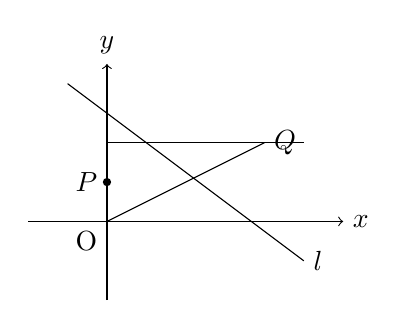
\begin{tikzpicture}
\draw[->] (-1,0) -- (3,0) node[right]{$x$};
\draw[->] (0,-1) -- (0,2) node[above]{$y$};
\draw (0,1) -- (2.5,1); 
\draw (0,0) -- (2,1) node[right]{$Q$};
\draw (-0.5,1.75) -- (2.5,-0.5) node[right]{$l$};
\fill (0,0.5) circle (1.5pt) node[left]{$P$};
\node at (0,0) [below left] {O};
\end{tikzpicture}
\end{center}

\subsection*{第4問}
[解] (1) $y=1$の時. $x=1$となり $Z^2 - Z + 2 = 0$ だが, これをみたす $Z \in \mathbb{Z}$ はない.

$1^\circ \ y=2$
$x=1$の時, $Z^2 - 2Z + 5 = 0$ となり, これをみたす $Z$ はない
$x=2$ " $Z^2 - 4Z + 8 = 0$ "

$2^\circ \ y=3$
$x=1$の時, $Z^2 - 3Z + 10 = 0$ "
$x=2$ " $Z^2 - 6Z + 13 = 0$ "
$x=3$ " $Z^2 - 9Z + 18 = 0$ となり, $Z=3, 6$ が適する.

以上から, $(x, y, Z) = (3, 3, 3), (3, 3, 6)$ (終)

(2) $a^2 + b^2 + c^2 = abc, \quad a \le b \le c \quad \cdots$ ① とする. $Z = bc - a$ とすると,
\[ bc - a \ge c \iff (b - 1)c \ge a \]
で, (1)から $b \ge 3$ だから, これは必ず成立し,
\begin{align*}
b^2 + c^2 + Z^2 &= b^2 + c^2 + (b^2c^2 + a^2 - 2abc) \\
&= b^2c^2 - abc = bcZ
\end{align*}
から $b^2 + c^2 + Z^2 = bcZ$ も成立. よって $(b, c, bc - a)$ は (A) をみたす. よって示された. (終)

(3) 漸化式 $\{a_n\}, \{b_n\}, \{c_n\}$ を,
\[ \begin{cases} a_{n+1} = b_n \\ b_{n+1} = c_n \\ c_{n+1} = b_n c_n - a_n \\ a_1 = b_1 = c_1 = 3 \end{cases} \quad \cdots * \]
によって定めると,
\[ c_{n+1} - c_n = (b_n - 1)c_n - a_n > c_n - a_n \ge 0 \quad (\because b_n \ge 3) \]
だから $c_{n+1} > c_n$ となる. つまり, $*$ で生成される $(a_n, b_n, c_n)$ は $n$ によって異なり, かつ (2) から (A) をみたす. よって (A) をみたす $(x, y, z)$ は無数にある. (終)

\subsection*{第5問}
[解] $\begin{cases} b_1 = 2 \\ b_{n+1} = b_n + \frac{1}{b_n} + 2 \end{cases} \quad \cdots$ ①

(1) $b_n > 2n \quad (n \ge 2) \quad \cdots \Diamond$ を帰納法で示す. $n=2$ の時, ①から $b_2 = 4 + \frac{1}{2}$ なので $\Diamond$ は成立. $n=k \in \mathbb{N}_{\ge 2}$ での成立をカテイすると, ①から
\[ b_{k+1} = b_k + \frac{1}{b_k} + 2 > 2(k + 1) \]
となり, $n=k+1$ でも $\Diamond$ は成立. よって示された. (終)

(2) (1) から $n \ge 2$ に対して $\frac{1}{a_n} > 2n \ \therefore \ a_n < \frac{1}{2n}$ である. $n \to \infty$ をかんがえるので $n$ は十分大きいとして良く, 右図で面積比較して,
\begin{align*}
\frac{1}{n} \sum_{k=1}^n a_k &< \frac{1}{n} \left( \frac{1}{2} + \sum_{k=2}^n \frac{1}{2k} \right) < \frac{1}{2n} \left( 1 + \int_1^n \frac{1}{x} dx \right) \\
\therefore \ \frac{1}{n} \sum_{k=1}^n a_k &< \frac{1 + \log n}{2n} \to 0 \quad (n \to \infty)
\end{align*}
から, $0 < a_k$ とあわせて ($\because$ ①から帰納的に $0 < a_k$), はさみうちから,
\[ \frac{1}{n} \sum_{k=1}^n a_k \to 0 \quad (\text{終}) \]

\begin{center}
\begin{tikzpicture}
\draw[->] (0,0) -- (3,0) node[right]{$x$};
\draw[->] (0,0) -- (0,2) node[above]{$y$};
\draw[domain=0.5:2.5, smooth] plot (\x, {1/\x});
\draw (1,0) rectangle (1.5, 1);
\draw (1.5,0) rectangle (2, 0.66);
\node[below] at (1,0) {$1$};
\node[below] at (2,0) {$n$};
\node at (0,1) [left] {$\frac{1}{a_n}$}; % rough inclusion based on scratch
\end{tikzpicture}
\end{center}

(3) ①から,
\[ b_{n+1} - b_n = 2 + a_n \]
$n=1, 2, \cdots, N$ として足して,
\[ b_{N+1} - b_1 = 2N + \sum_{k=1}^N a_k \]
両辺 $N+1$ でわって,
\[ \frac{1}{(N+1)a_{N+1}} = \frac{2}{N+1} + 2\frac{N}{N+1} \cdot \frac{1}{N} \sum_{k=1}^N a_k \xrightarrow{N \to \infty} 2 \quad (\because (2)) \]
だから, $0 < x$ で $\frac{1}{x}$ が連続なことから,
\[ N a_N \to \frac{1}{2} \quad (N \to \infty) \quad (\text{終}) \]

[解2]
(3) $b_n \le 2n + \log n$ を帰納法で示す. $n=1$ の時は成立するので, $1 \le n = k \in \mathbb{N}$ での成立をカテイ. ①から
\[ b_{k+1} = b_k + \frac{1}{b_k} + 2 \le 2(k+1) + \log k + \frac{1}{2k} \quad (\because 2k \le b_k) \quad \cdots \text{②} \]
ここで, $f(x) = \log(x+1) - \log x - \frac{1}{2x}$ とすると,
\[ f'(x) = \frac{1}{x+1} - \frac{1}{x} + \frac{1}{2x^2} = \frac{1-x}{2x^2(x+1)} \]
から増減表をうる
\begin{center}
\begin{tabular}{|c|c|c|c|c|}
\hline
$x$ & $0$ & $\cdots$ & $1$ & $\cdots$ \\ \hline
$f'(x)$ & & $+$ & $0$ & $-$ \\ \hline
$f(x)$ & & $\nearrow$ & & $\searrow$ \\ \hline
\end{tabular}
\end{center}
$\left( \text{$x \to \infty$ の時, 平均値から $x < c < x+1$ なる $c$ に対し, } f(x) = \frac{1}{c} - \frac{1}{2x} > \frac{1}{x+1} - \frac{1}{2x} > 0 \right)$

よって $1 \le x$ では $f(x) > 0$ つまり $\log(k+1) > \log k + \frac{1}{2k}$ だから, ②より
\[ b_{k+1} \le 2(k+1) + \log(k+1) \]
よって $n=k+1$ でも成立. 以上から成立し,
\[ 2n < \frac{1}{a_n} < 2n + \log n \]
だから, はさみうちより $n a_n \to \frac{1}{2}$ (終)

\subsection*{第6問}
[解] $t = e^x$ とおく. $x > 0$ から $t > 1$ である.

(1) 
\[ f'(x) = \frac{dt}{dx} \frac{df}{dt} = t \cdot \left\{ \frac{12(t^2 - 3t)}{(t^2 - 1)} \right\}' = 12t \cdot \frac{t^4 + 3}{(t^2 - 1)^2} > 0 \quad (\because t > 1) \]
だから $f(x)$は単調増加. これと $f(x) = 12 \frac{t - 3/t}{1 - 1/t^2} \xrightarrow{x \to \infty} \infty \quad (\because t \to \infty)$,
$f(x) = 12 \frac{t(t^2 - 3)}{(t+1)(t-1)} \xrightarrow{x \to +0} -\infty \quad (\because t \to 1+0)$ から, 任意の定数 $a$ に対し $f(x) = a$ なる $x > 0$ がただ1つある. (終)

(2) グラフの概形は右図で求める面積 $S$ は斜線部.
\begin{align*}
f(x) = 8 &\iff 3t^3 - 2t^2 - 9t + 2 = 0 \\
&\iff (t - 2)(3t^2 + 4t - 1) = 0 \\
&\therefore t = 2 \quad (\because t > 1) \\
f(x) = 27 &\iff 4t^3 - 9t^2 - 12t + 9 = 0 \\
&\iff (t - 3)(4t^2 + 3t - 3) = 0 \\
&\therefore t = 3 \quad (\because t > 1)
\end{align*}
だから,
\[ S = 27 \log 3 - 8 \log 2 - \int_{\log 2}^{\log 3} f(x) dx \quad \cdots \text{①} \]
となる. ここで,
\begin{align*}
\int_{\log 2}^{\log 3} f(x) dx &= \int_2^3 \frac{12(t^3 - 3t)}{t^2 - 1} \frac{1}{t} dt \\
&= 12 \int_2^3 \frac{t^2 - 3}{t^2 - 1} dt = 12 \int_2^3 \left( 1 - \frac{1}{t - 1} + \frac{1}{t + 1} \right) dt \\
&= 12 \Big[ t - \log(t-1) + \log(t+1) \Big]_2^3 \\
&= 12(1 + \log 2 - \log 3) \quad \cdots \text{②}
\end{align*}
だから, ②を①に代入して
\[ S = 39 \log 3 - 20 \log 2 - 12 \quad (\text{終}) \]

[解2]
(2) $S = \int_8^{27} g(x) dx$ とおく. $x = f(y)$ なる置換をして,
\begin{align*}
S &= \int_{\log 2}^{\log 3} y \cdot \frac{df(y)}{dy} dy \\
&= \int_{\log 2}^{\log 3} y \cdot f'(y) dy \\
&= \Big[ y f(y) \Big]_{\log 2}^{\log 3} - \int_{\log 2}^{\log 3} f(y) dy \\
&= 27 \log 3 - 8 \log 2 - \int_{\log 2}^{\log 3} f(y) dy
\end{align*}
(以下同文)

\begin{center}
\begin{tikzpicture}
\draw[->] (0,0) -- (4,0) node[right]{$x$};
\draw[->] (0,-1) -- (0,4) node[above]{$y$};
\draw[domain=1.5:3.5, smooth] plot (\x, {\x*1.2 - 1}) node[right]{$y=f(x)$};
\draw[dashed] (0,1) node[left]{$8$} -- (1.66,1) -- (1.66,0) node[below]{$\log 2$};
\draw[dashed] (0,3) node[left]{$27$} -- (3.33,3) -- (3.33,0) node[below]{$\log 3$};
\node at (1,0) [below] {$(\frac{1}{2}\log 3)$};
\fill[pattern=north east lines] (0,1) -- (1.66,1) -- (3.33,3) -- (0,3) -- cycle;
\end{tikzpicture}
\end{center}

\end{document}
